% !TeX root = ../main.tex

\chapter{Evaluation}\label{chapter:evaluation}
To verify the capability of the approach proposed in this work, the prototypical implementation was evaluated.
The idea is to find out, whether the approach is capable of detecting copied code in a codebase and, by that, unveil license infringements.
For that purpose, 2000 GPL licensed projects were indexed using the prototypical implementation of the tool.
After that, other open source projects, which are licensed not compatible with GPL and therefore should not contain any of the GPL licensed code indexed before, where analyzed and resulting matches categorized.
This chapter describes the test setup evaluates timings, database sizes and findings.

\section{Test Setup}\label{section:evaluation/test_setup}
As a source for most of the target projects, GitHub was chosen, only Teamscale is a closed source project.
GitHub's REST API was used to generate a list of 1.000 GPL licensed Java and 1.000 GPL licensed C or C++ projects.
All of the projects were checked out locally resulting in sizes as shown in \autoref{table:locs}.
Indexing those 2.000 projects including their history took 15h on a consumer laptop with 16 GB of RAM and an Intel i7 CPU with 4 cores and hyper-threading.
The indexing was done independently for Java and C/C++ generating two databases.
The resulting database sizes are 4 GB for Java and 33 GB for C/C++, the Bloom filter's sizes are 55 MB and 147 MB for Java and C/C++.
Inspection of several indexed projects showed, the huge difference for the sizes can be justified in the amount of actual code in the repositories.
It seems like Java projects contain more images, binary files or other resources, compared to the C/C++ projects.

\begin{table}[ht]
	\centering
	\begin{tabular}{l|rrrrr}
		& \textbf{Scanned Files} & \textbf{Lines of Code} & \textbf{Total size} & \textbf{Hashes} & \textbf{Chunks} \\ 
		\hline 
		Java & 836.555 & 57.834.764 & 94 GB & 23.773.065 & 35.069.633 \\
		C/C++ & 1.023.092 & 380.338.327 & 102 GB & 61.349.163 & 221.315.454 \\ 
	\end{tabular}
	\caption{Sizes of the 2.000 indexed projects}\label{table:locs}
\end{table}

After two weeks, the index was updated for both Java and C/C++ as described in \autoref{section:implementation/history_analysis/update}.
Approximately one third of the reference projects contained one or more new tags which were indexed.
The update took a total of one hour including calculation of the Bloom filter.

After indexing those projects, several other projects, licensed not compatible with GPL, where analyzed for matches using the approach described in \autoref{section:implementation/finding_matches}.
The selected projects are mostly large standalone programs or frameworks, which are not library code.
\autoref{table:target_projects} shows the chosen target projects, their license and the lines of code of files written in the corresponding language.
To reduce the amount of irrelevant matches, generated code, third party code and libraries were excluded from the target projects during analysis, by instructing the analysis to exclude corresponding directories of the target projects.

\begin{table}[ht]
	\centering
	\begin{tabular}{l|llr}
		& \textbf{Name} & \textbf{License} & \textbf{Lines of Code} \\
		\hline 
		\parbox[t]{2mm}{\multirow{10}{*}{\rotatebox[origin=c]{90}{JAVA}}} 
		& IntelliJ IDEA & Apache 2.0 & 3.500.000 \\
		& Eclipse JDT Core & Eclipse Public License & 1.459.000 \\
		& Elasticsearch & Apache 2.0 & 711.000 \\
		& Eclipse JDT UI & Eclipse Public License & 685.000 \\
		& Facebook Buck & Apache 2.0 & 597.000 \\
		& Teamscale & Closed Source & 480.000 \\
		& Spring Boot & Apache 2.0 & 223.000 \\
		& Openfire & Apache 2.0 & 200.000 \\
		& Killbill & Apache 2.0 & 150.000 \\
		& JabRef & MIT & 125.000 \\
		\hline 
		\parbox[t]{2mm}{\multirow{10}{*}{\rotatebox[origin=c]{90}{C/C++}}} 
		& Chromium & BSD License 2.0 & 4.651.000 \\
		& ArangoDB & Apache 2.0 & 4.855.000 \\
		& Tensorflow & Apache 2.0 & 662.000 \\
		& Apple Swift & Apache 2.0 & 520.000 \\
		& Mesos & Apache 2.0 & 309.000 \\
		& Apache httpd & Apache 2.0 & 214.000 \\
		& RethinkDB & Apache 2.0 & 201.000 \\
		& Tesseract & Apache 2.0 & 147.000 \\
		& Bitcoin & MIT & 119.000 \\
		& Electron & MIT & 67.000 \\
	\end{tabular}
	\caption{Target projects used for testing, their license and LOCs in the corresponding language}\label{table:target_projects}
\end{table}

\section{Hash Filter Performance}\label{section:evaluation/hash_filter_performance}
The Bloom filter can return false positives, thus, matches are expected even if no code has been copied from a reference project into the target project for large enough projects.
Those matches - called false positive filter matches (FPFM) in the remainder of this work - are expected to occur once for roughly every 10.000 statements in the target project, since the probability for a false positive of the Bloom filter is calculated to be 0,01\%. 

\autoref{table:unfiltered_findings} lists results regarding amount of analyzed chunks as well as false and true positive matches.
Columns are defined as follows:
\begin{description}
	\item[Target System] The name of the target system
	\item[Files] Number of files of the target project, which match the corresponding language (Java or C/C++) and are therefore analyzed.
	\item[Chunks] Resulting amount of chunks extracted from the target system.
	\item[FPFM] False Positive Filter Matches as described above.
	\item[True Positives] Amount of actual matches, which could be found in the index and their relative amount in comparison to all chunks extracted from the target system.
	\item[Requests] Amount of requested match details. Note here that files with less than two matches are ignored as described in \autoref{section:implementation/finding_matches}.
\end{description}

\begin{table}[ht]
	\centering
	\begin{tabular}{l|lrrrrr}
		 & \textbf{Target System} & \textbf{Files} & \textbf{Chunks} & \textbf{FPFM} & \textbf{True Positives} & \textbf{Requests} \\ 
		\hline 
		\parbox[t]{2mm}{\multirow{10}{*}{\rotatebox[origin=c]{90}{JAVA}}} 
		& IntelliJ IDEA & 35.398 & 1.570.170 & 183 & 8.134 (0,5\%) & 8.035 \\
		& Eclipse JDT Core & 1.829 & 267.130 & 29 & 510 (0,2\%) & 509 \\
		& Elasticsearch & 5.560 & 414.448 & 45 & 1.105 (0,3\%) & 1.004 \\
		& Eclipse JDT UI & 2.736 & 274.040 & 29 & 482 (0,2\%) & 444 \\
		& Buck & 5.150 & 261.605 & 21 & 575 (0,2\%) & 548 \\
		& Teamscale & 5.463 & 185.648 & 21 & 458 (0,2\%) & 434 \\
		& Spring Boot & 3.756 & 94.935 & 11 & 1.010 (1,1\%) & 967 \\
		& Openfire & 1.572 & 121.775 & 15 & 2.106 (1,7\%) & 2.084 \\
		& Killbill & 1.477 & 79.118 & 13 & 550 (0,7\%) & 539 \\
		& JabRef & 1.389 & 72.052 & 5 & 204 (0,3\%) & 183 \\
		\hline 
		\parbox[t]{2mm}{\multirow{10}{*}{\rotatebox[origin=c]{90}{C/C++}}} 
		& Chromium & 14.241 & 364.126 & 53 & 16.951 (4,7\%) & 16.912 \\
		& ArangoDB & 1.096 & 135.291 & 8 & 571 (0,4\%) & 569 \\
		& Tensorflow & 1.207 & 50.382 & 3 & 59 (0,2\%) & 56 \\
		& Apple Swift & 848 & 56.386 & 11 & 14 (0,0\%) & 13 \\
		& Mesos & 341 & 64.090 & 6 & 18 (0,0\%) & 15 \\
		& Apache httpd & 529 & 126.936 & 18 & 949 (0,7\%) & 949 \\
		& RethinkDB & 91 & 8.664 & 0 & 2.906 (33,5\%) & 2.905 \\
		& Tesseract & 559 & 82.946 & 10 & 27 (0,0\%) & 29 \\
		& Bitcoin & 491 & 57.847 & 5 & 97 (0,2\%) & 97 \\
		& Electron & 342 & 6.846 & 1 & 0 (0,0\%) & 0 \\
	\end{tabular}
	\caption{Amount of files and chunks as well as true and false positives caused by the hash filter and the resulting requested chunk details}\label{table:unfiltered_findings}
\end{table}

This result shows that the hash filter is reducing the required lookups to a fraction.
Load on the server can be greatly reduced and analysis of a target system's code therefore is a lot quicker.
The analysis took less than 20 seconds even for the biggest projects not including networking.
In a real world scenario, this will be slower, since communication with the server will add additional delays.
Requesting the locations for each hash passing the hash filter individually, causes a lot of requests with high overhead caused by creating single network packets.
Additional authentication on the server may be required to control access further slowing down the analysis.
Instead, sending hashes in batches may be a better solution.

\newpage
\section{Detection of License Infringements}\label{section:evaluation/detecting_infringements}
As the previous section shows, matches have to be filtered, in order to remove false positives and matches, which are not relevant in the context of license infringement.
Aggregation and filtering is done as described in \autoref{section:implementation/finding_matches}.
Based on the license definitions in \autoref{section:preliminaries/infringement/relevant_licenses}, each match is manually inspected and grouped into one of the following categories:
\begin{description}
	\item [Accidential Clones (AC)]
		Matches which are similar by \glqq accident\grqq, e.g. generated code, interface implementations, declarations of structs/enums, switch-case blocks, table data especially present in C/C++.
	\item[Otherwise Licensed Code (OLC)]
		Code which is actually copied from the reference project or originates from a common source licensed under a permissive license or is public domain.
		If the copied code is under permissive license (e.g. MIT licensed code copied into the reference project), attribution is done correcty and therefore, this is not a license infringement.
		Note here that code can also be copied into the reverse direction in the context of this evaluation, since analyzed target projects are licensed in a way, where they can be copied to GPL licensed code with attribution.
	\item[Copied, but not Attributed (CNA)]
		This marks the use of permissive licenses and therefore is the same as otherwise licensed code, but not attributed correctly by the target project.
		The severity of the violation is depending on the license of the source, the length of the copied segment and its similarity.
		Those violations can be fixed by correctly attributing the source of the code.
	\item[License Infringement (LI)]
		Code which has been copied from a reference system licensed under a restrictive license and is violation due to the target's license.
\end{description}

AC can be seen as a false positive of the approach, whereas OLC detects code, which has been copied, but the license of the code is not violated.
Even though OLC does not violate a license, detection of such code still may be of interest, since using a library instead of copying the code into the codebase can be the better alternative \cite{heinemann2012effective}.
In general, those two cases are not marking violations.

CNA on the other hand, marks a violation of the license, because the code has not been attributed correctly, but the significance of such a violation may not be very high.
Copied code categorized as LI may even be attributed correctly, but still is a violation of the copied code's license.

\subsection{Counting Matches}
A scanned target system file can have multiple matches for a chunk, since clones also exist between and within reference systems.
Therefore, in the following evaluation, matches are counted on the target file and only the most relevant concatenated matches of the reference files are regarded.
\autoref{table:scan_results} shows the results of manually categorizing each match.
A match is a relation between a file of the target system to the best match of a file in a reference system, indicating a high similarity.

If a target file has multiple sections of copied code, which \textit{does not overlap} and is from multiple other files (e.g. common in utils code), each match in the target file is counted once.
\autoref{fig:match_counting} shows an example, where multiple sections of code are copied from \texttt{Reference File 1} to the \texttt{Target File}.
This is counted as one match.
There is also one coherent block of code copied from \texttt{Reference File 2} to the \texttt{Target File}, which is also counted as a match.
The resulting total count of matches for the \texttt{Target File} in this example is two.

\begin{figure}[h]
	\centering
	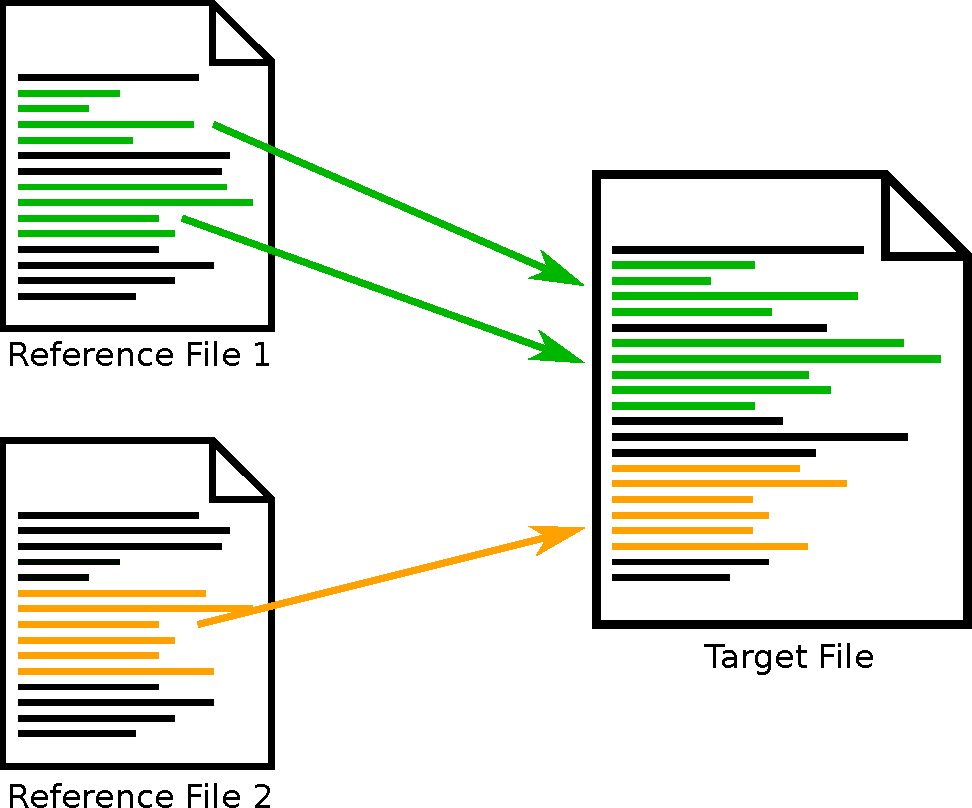
\includegraphics[width=0.7\linewidth]{figures/match_counting.pdf}
	\caption{Illustration of match counting}\label{fig:match_counting}
\end{figure}

\newpage
\subsection{Results and Findings}
The results in \autoref{table:scan_results} are twofold.
On the one hand, it shows that finding license infringements is possible.
On the other hand, the amount of overall detected matches prevails the amount of relevant matches by far.
This is due to many accidental clones (AC), which are caused by e.g. interface implementations or tables, as well as otherwise licensed code (OLC) due to the fact that most licenses of target projects allow copying of code into a codebase licensed under GPL.
Therefore, many of the hits for OLC are caused by code of the target project being found in the reference project.

\begin{table}[ht]
	\centering
	\newcolumntype{R}[1]{>{\raggedleft\arraybackslash}p{#1}}
	\begin{tabular}{l | l rrrr}
		& \textbf{Name} & \textbf{AC} & \textbf{OLC} & \textbf{CNA} & \textbf{LI} \\
		\hline 
		\parbox[t]{2mm}{\multirow{10}{*}{\rotatebox[origin=c]{90}{JAVA}}} 
		& IntelliJ IDEA & 86 & 21 & 11 & 7 \\
		& Eclipse JDT Core & 17 & 8 & 0 & 0 \\
		& Elasticsearch & 13 & 3 & 4 & 3 \\
		& Eclipse JDT UI & 3 & 19 & 0 & 0 \\
		& Facebook Buck & 11 & 7 & 0 & 0  \\
		& Teamscale & 12 & 3 & 1 & 2 \\
		& Spring Boot & 19 & 6 & 0 & 0 \\
		& Openfire & 20 & 9 & 5 & 0 \\
		& Killbill & 20 & 2 & 0 & 0 \\
		& JabRef & 3 & 2 & 0 & 1 \\
		\hline 
		\parbox[t]{2mm}{\multirow{10}{*}{\rotatebox[origin=c]{90}{C/C++}}} 
		& Chromium & 16 & 429 & 0 & 0 \\
		& ArangoDB & 1 & 5 & 0 & 0 \\
		& Tensorflow & 2 & 0 & 0 & 0 \\
		& Apple Swift & 2 & 0 & 0 & 0 \\
		& Mesos & 1 & 0 & 0 & 0 \\
		& Apache httpd & 5 & 13 & 0 & 0 \\
		& RethinkDB & 0 & 29 & 0 & 0 \\
		& Tesseract & 2 & 1 & 0 & 0 \\
		& Bitcoin & 0 & 6 & 0 & 0 \\
		& Electron & 0 & 0 & 0 & 0 \\
	\end{tabular}
	\caption{Target projects and categorized matches}\label{table:scan_results}
\end{table}

\subsubsection*{General Findings}
For Java, the approach found several infringements, for C/C++ no LI nor CNA were found.
This may be explained, by many of the C/C++ target projects being of organizations, which have their own library codebase.
Manual investigation in the findings leave the impression that C/C++ developers are more careful in copying code correctly and attributing copied code correctly.

Sometimes, the decision whether a match is actually copied code (OLC or CNA depending on the license) or just accidential clones (AC) is visible in the comments.
When both sides have a high similarity in the comments, the probability for the code being copied increases significantly.
Still, removing comments when normalizing code for comparison is advisable, since comments often are removed or added.

The match supplied by the tool sometimes was not the actual origin of the code.
However in many cases, the suggested matches could give hints on the origin of the code and combined with further searching the Internet, the originating source could be determined.
This process is very hard to automate and manual inspection is required nonetheless, since the severity of the infringement has to be assessed.
For some rare cases, even searching for implementations of the specific problem on the Internet did not help in finding the originating source.
For such cases, the code was seen as CNA, since no attribution was made and the code may be a potential infringement.
This also shows that indexing one reference project often includes several other projects (with different licenses), since sometimes, dependencies are copied into the codebase of a reference project.

Infringements not only could be found in the target system.
Sometimes, the original file header was replaced by the GPL header of the reference system, which removes the attribution and thus results in a violation for many licenses.
Those cases are not regarded in this test, but still show that the problem targeted in this work exists.

\subsubsection*{Accidential Clones (AC)}
Mostly, AC findings are caused by interface implementations, structs and enumerations used for communication with APIs or table definitions.
One example of a common AC is shown in \autoref{fig:ac}.
Here, the Java specific \texttt{hashCode} and \texttt{equals} methods cause a match.
Method generators supplied by the used IDE may have caused the high similarity.
\begin{figure}[htpb]
	\centering
	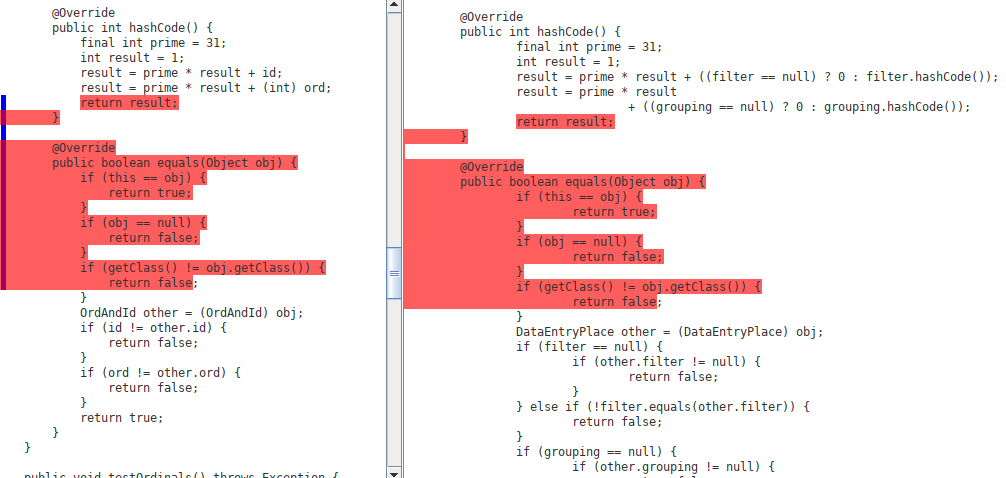
\includegraphics[width=\linewidth]{figures/ac.png}
	\caption{Example for AC. Left target, right reference code}
	{
		\begin{flushleft}
			\tiny Sources:\\
			\textbf{Left:}
			\href{https://github.com/elastic/elasticsearch/blob/b1039164a11cd2e9968ac61c7260997eaa9f480a/core/src/test/java/org/elasticsearch/index/fielddata/ordinals/MultiOrdinalsTests.java}{https://github.com/elastic/elasticsearch/blob/b1039164a11cd2e9968ac61c7260997eaa9f480a/core/src/test/java/org/elasticsearch/ index/fielddata/ordinals/MultiOrdinalsTests.java}\\
			\textbf{Right:}
			\href{https://github.com/bedatadriven/activityinfo/blob/1b4f3cc73e9186a93178c8354925dcf0ebc68ff5/sigmah/src/main/java/org/sigmah/client/page/entry/place/DataEntryPlace.java}{https://github.com/bedatadriven/activityinfo/blob/1b4f3cc73e9186a93178c8354925dcf0ebc68ff5/sigmah/src/main/java/org/sigmah/client/ page/entry/place/DataEntryPlace.java}
		\end{flushleft}
	}
	\label{fig:ac}
\end{figure}

\newpage
\subsubsection*{Otherwise Licensed Code (OLC)}
OLC had many matches both for Java and C/C++.
Either code was attributed correctly like the example in \autoref{fig:olc_attributed} or the code can be copied without attribution like in the case of code under public domain like the example in \autoref{fig:olc_public_domain} shows.
Findings like those are not license infringements.
However, they may be of interest, since third party code can be monitored and code could be linked instead of copied.

A reference system being licensed under a specific license does not cause all code files of that system are actually licensed as such.
Resolving the actual license of a file can be very hard, since headers often do not contain any information on the file's license.

Some of the selected reference projects are forks of one of the target projects.
Examples are Eclipse JDT Core and the Overture tool\footnote{\href{https://github.com/overturetool/overture}{https://github.com/overturetool/overture} (09.01.2018)} or Chromium and the OBS Studio project\footnote{\href{https://github.com/jp9000/obs-studio}{https://github.com/jp9000/obs-studio} (09.01.2018)}.
Almost all matches of RethinkDB were caused by copied code from RapidJSON\footnote{\href{https://github.com/Tencent/rapidjson}{https://github.com/Tencent/rapidjson} (09.01.2018)}.

\begin{figure}[h!]
	\centering
	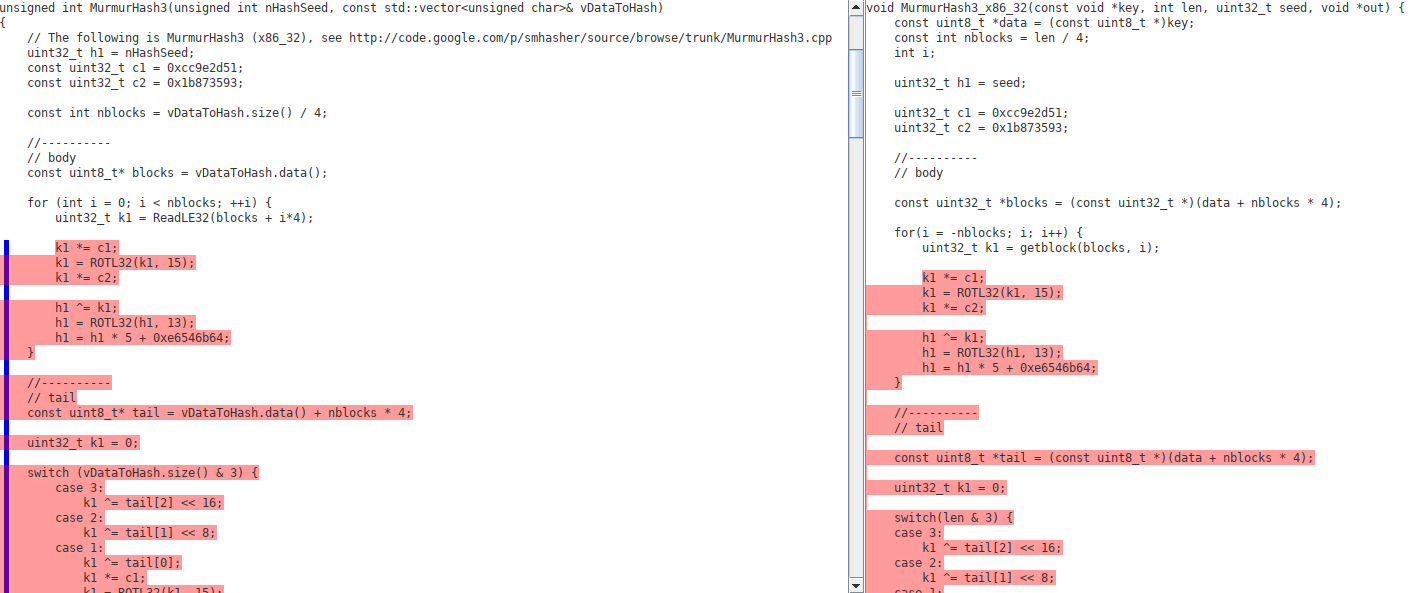
\includegraphics[width=\linewidth]{figures/olc_public_domain.png}
	\caption{Example for public domain code being categorized as OLC. Left target, right reference code}
	{
		\begin{flushleft}
			\tiny Sources:\\
			\textbf{Left:}
			\href{https://github.com/bitcoin/bitcoin/blob/5d132e8b974652d96466a1b73ec1231614719fe2/src/hash.cpp}
			{https://github.com/bitcoin/bitcoin/blob/5d132e8b974652d96466a1b73ec1231614719fe2/src/hash.cpp}\\
			\textbf{Right:}
			\href{https://github.com/sahib/rmlint/blob/e1a64fefd26f32616fdb75c75c55aa1782c1d8f5/lib/checksums/murmur3.c}
			{https://github.com/sahib/rmlint/blob/e1a64fefd26f32616fdb75c75c55aa1782c1d8f5/lib/checksums/murmur3.c}
		\end{flushleft}
	}

	\label{fig:olc_public_domain}
\end{figure}

\newpage
\begin{figure}[h!]
	\centering
	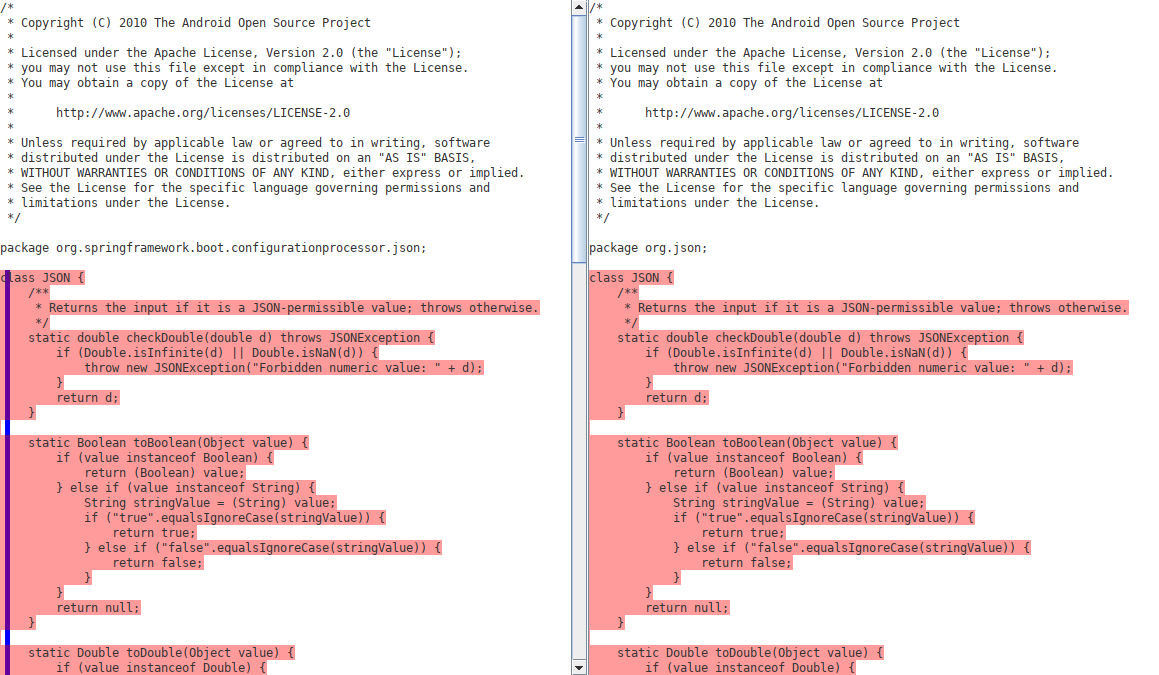
\includegraphics[width=\linewidth]{figures/olc_attributed.png}
	\caption{
		Example for correctly attributed OLC. Left target, right reference code
	}{
		\begin{flushleft}
			\tiny Sources:\\
			\textbf{Left:}
			\href{https://github.com/spring-projects/spring-boot/blob/ac004eabf35af2a11cbeb19e31717b70df6224f7/spring-boot-project/spring-boot-tools/spring-boot-configuration-processor/src/main/java/org/springframework/boot/configurationprocessor/json/JSON.java}
			{https://github.com/spring-projects/spring-boot/blob/ac004eabf35af2a11cbeb19e31717b70df6224f7/spring-boot-project/spring-boot-tools/spring-boot-configuration-processor/src/main/java/org/springframework/boot/configurationprocessor/json/JSON.java}\\
			\textbf{Right:}
			\href{https://github.com/projectestac/jclic/blob/bb94af09efbe6cf932472f6b285931f1d04291fb/extensions/json/src/org/json/JSON.java}
			{https://github.com/projectestac/jclic/blob/bb94af09efbe6cf932472f6b285931f1d04291fb/extensions/json/src/org/json/JSON.java}
		\end{flushleft}
	}
	\label{fig:olc_attributed}
\end{figure}

\newpage
\subsubsection*{Copied but not Attributed Code (CNA)}
In many cases, attributing the origin of copied code is not done correctly, as manual inspection showed.
\autoref{fig:cna} shows an example for CNA, where hundreds of lines were copied, but no attribution was made.
The original file header containing the license information including the terms and conditions was replaced by the target project's file header.
This causes a violation of the licenses terms, since attribution has to be made according to the reference file's license.
\begin{figure}[htpb]
	\centering
	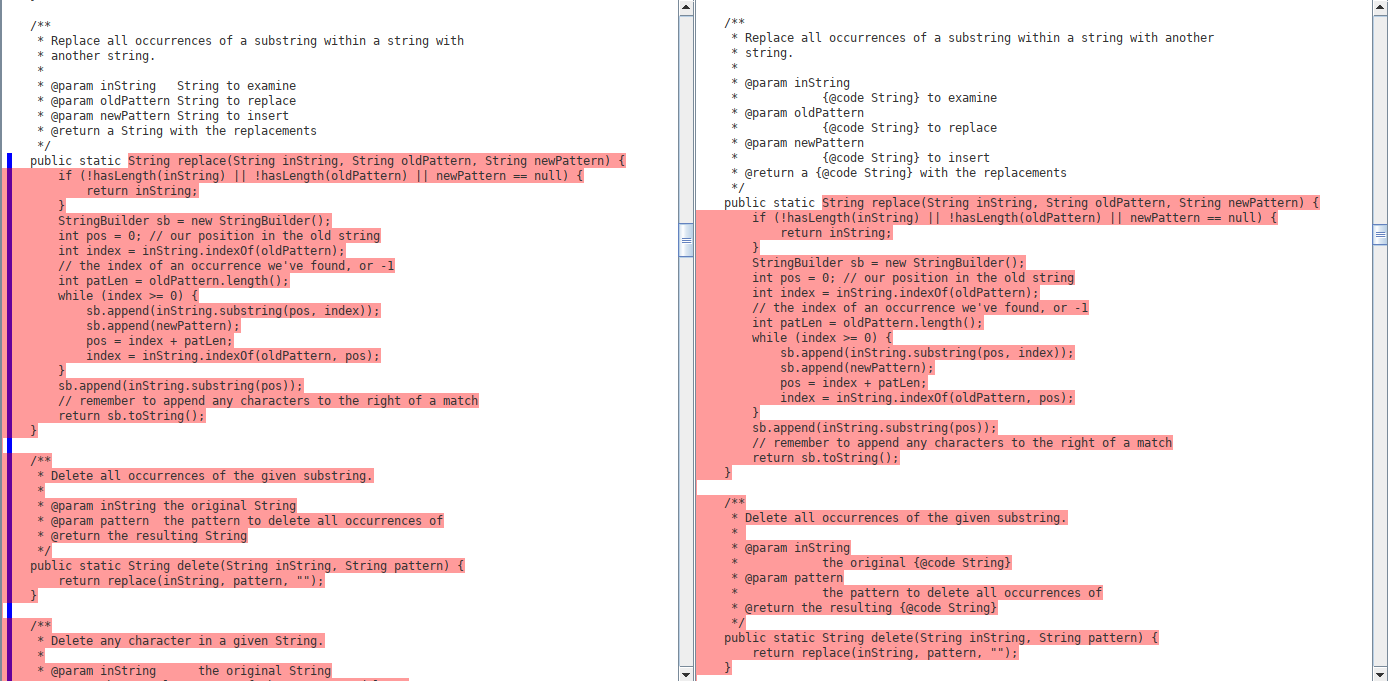
\includegraphics[width=\linewidth]{figures/cna.png}
	\caption{Example for CNA. Left target, right reference code}
	{
		\begin{flushleft}
			\tiny Sources:\\
			\textbf{Left:}
			\href{https://github.com/elastic/elasticsearch/blob/b1039164a11cd2e9968ac61c7260997eaa9f480a/core/src/main/java/org/elasticsearch/common/Strings.java}{https://github.com/elastic/elasticsearch/blob/b1039164a11cd2e9968ac61c7260997eaa9f480a/core/src/main/java/org/elasticsearch/common/Strings.java}\\
			\textbf{Right:}
			\href{https://github.com/HotswapProjects/HotswapAgent/blob/2d55e7c0feb809e33c5cb2f384f8d993fb5562ed/hotswap-agent-core/src/main/java/org/hotswap/agent/util/spring/util/StringUtils.java}{https://github.com/HotswapProjects/HotswapAgent/blob/2d55e7c0feb809e33c5cb2f384f8d993fb5562ed/hotswap-agent-core/src/main/java/org/hotswap/agent/util/spring/util/StringUtils.java}
		\end{flushleft}
	}
	\label{fig:cna}
\end{figure}

\newpage
\subsubsection*{License Infringment (LI)}
Cases categorized as LI are violations of the GPL, where code is copied from a GPL licensed file to the target system.
Almost all cases found are caused by adoption of classes from the Java Development Kit (JDK).
The license of both, OpenJDK's and Oracle JDK's source code files is not compatible with permissive licenses like Apache or MIT, nor with closed source.
It seems like many developers are not aware of this.
On example of such an infringement can be found in \autoref{fig:li}, where a method of a class in the JDK was modified.
The code is then licensed under Apache 2.0 which is not compatible with GPL.
Instead, the code should be licensed under GPL.
This example shows that even small amounts of copied code which cause violations can be detected using the tool, although modifications were made.

Many of those cases are rather small and may not be prosecuted when uncovered.
Nonetheless, those findings show that many developers do not know how and which code can be copied without causing license infringements or just do not care about violating open source licenses.
\begin{figure}[htpb]
	\centering
	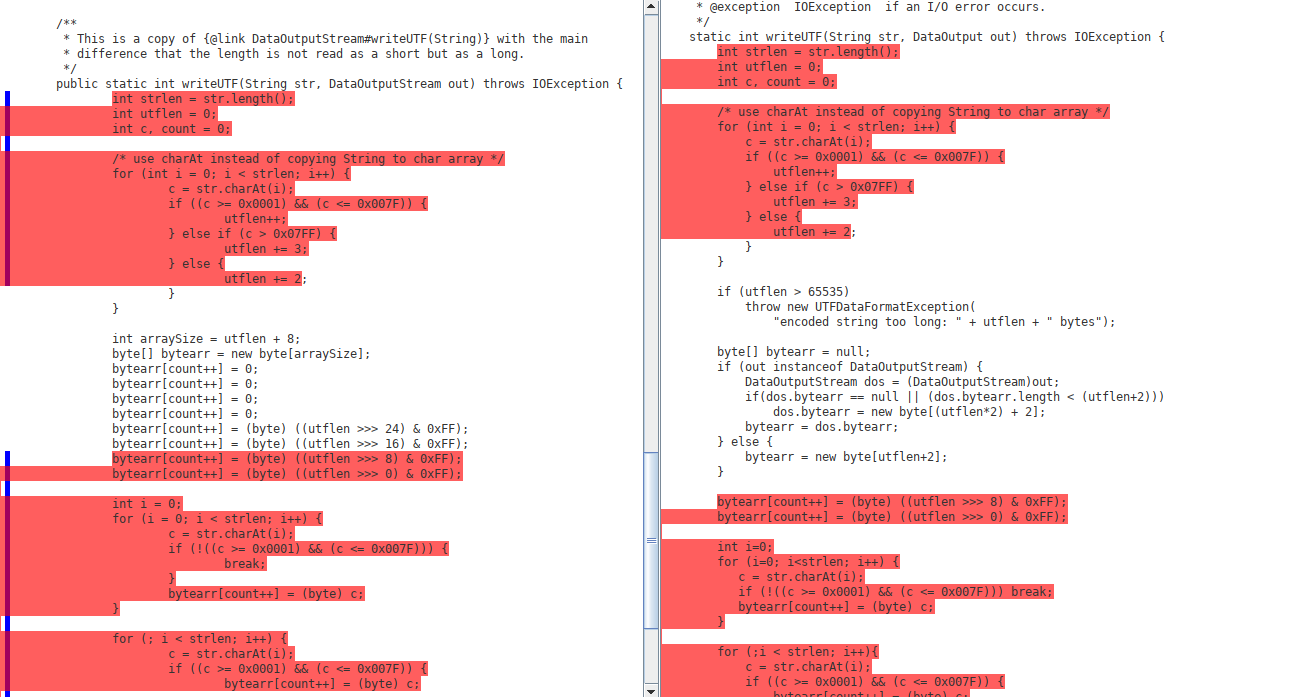
\includegraphics[width=\linewidth]{figures/li.png}
	\caption{Example for LI. Left target, right reference code}
	{
		\begin{flushleft}
			\tiny Sources:\\
			\textbf{Left:}
			Teamscale\\
			\textbf{Right:}
			\href{https://github.com/JetBrains/jdk8u_jdk/blob/2283b9d1d8f03fea8fa192c248b58726a66a6eaf/src/share/classes/java/io/DataOutputStream.java}{https://github.com/JetBrains/jdk8u\_jdk/blob/2283b9d1d8f03fea8fa192c248b58726a66a6eaf/src/share/classes/java/io/DataOutputStream.java}
		\end{flushleft}
	}
	\label{fig:li}
\end{figure}

\newpage
\subsection{Testing Recall}
Asserting the recall of clone detection tools is difficult.
Benchmarks like the work of Svajlenko et al. \cite{svajlenko2014towards} can give insight on the recall performance.
Analyzing this work with such a benchmark is beyond the scope of this work and may even be unsuitable, since the benchmark is testing for similar code constructs, which can be refactored for reuse to reduce redundancy and enhance software quality.
In contrast, the tool presented in this work tries to find code which has a high similarity and can be argued for being copied.

\section{Confidentiality}
The tool may be used for closed source target systems.
One key issue for companies is confidentiality regarding own source code.
Uploading code to a server maintained externally to the company may not be conform with the company's data privacy policies.

The approach presented in this work is only sending hashes which represent information relevant for identifying chunks.
In theory, this should restrict flow of information about the source code to a minimum and conclusions about the code can not be made.
However, when the code for a hash is known on the server side, i.e. a match for a hash is found, the server knows the code for the hash on the client.
If enough matches are found, the server may be able to reconstruct parts of the source code.
Still, information about the source code leaking from the client to the server is very limited.